\section{System Architecture}
A web application was developed to demonstrate the use of keyword search with ontology in an information retrieval (IR) system. This IR application consists of two components - one for crawling and indexing and the other for searching and viewing.

\subsection{Crawling and Indexing}
\label{subsec:crawl_and_index}
As defined by \citet{Manning2008}, Web crawling is the process by which we gather pages from the Web, in order to index them and support a search engine. In our context, more specifically, it means the process of gathering document data from the Document Server. The crawled text can then be fed into the search engine (Solr in our case) for indexing. Indexing is the process of constructing an inverted index.

Figure \ref{fig:comp_crawl_index} shows the component architecture for crawling and indexing. During the crawling step, the cleaned text and meta-data of each section would be fetched and stored into MySQL database. The cleaned text has all formulas, including numeric expressions, replaced with the placeholder \texttt{[FORMULA]}. The PDF documents for each section are also fetched and stored into the \texttt{Media} folder in the Application Server. As for the indexing step, the cleaned text and some meta-data stored in MySQL database would then be fed into Solr for indexing. Additional normalization, mentioned in Section \ref{subsec:solr_filters}, is done before indexing in Solr. 

\begin{figure}[!htbp]
  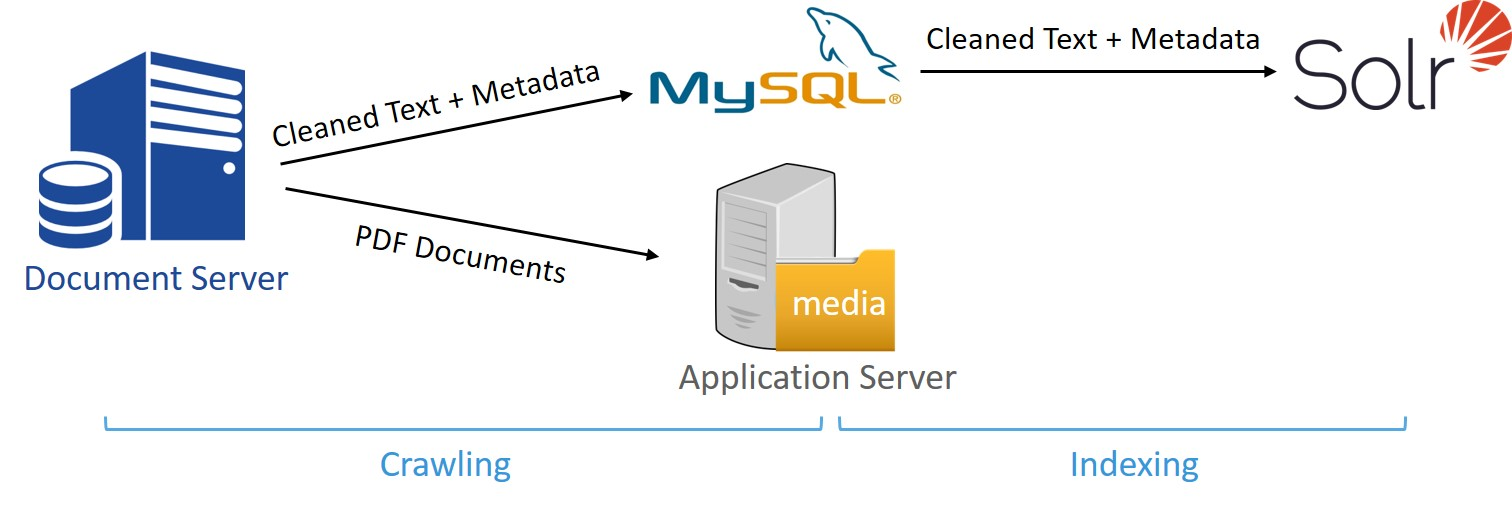
\includegraphics[width=.9\textwidth]{proposed_methodology_and_system_specifications/component_crawling_indexing.jpg}
  \caption{Component for Crawling and Indexing}
  \label{fig:comp_crawl_index}
\end{figure}

By right, term-to-concept mappings should have also been fetched and stored into MySQL database during crawling. However, since the concept recognition module has not been developed and is not part of the project scope, we had to manually fill some mappings data into MySQL database for demonstration purpose. The hierarchical concept ontology was also manually created in the same database.

\subsection{Searching and Viewing}
Figure \ref{fig:comp_search} shows the component architecture for searching and viewing. The interaction of different components for searching and viewing is elaborated below.

\begin{figure}[!htbp]
  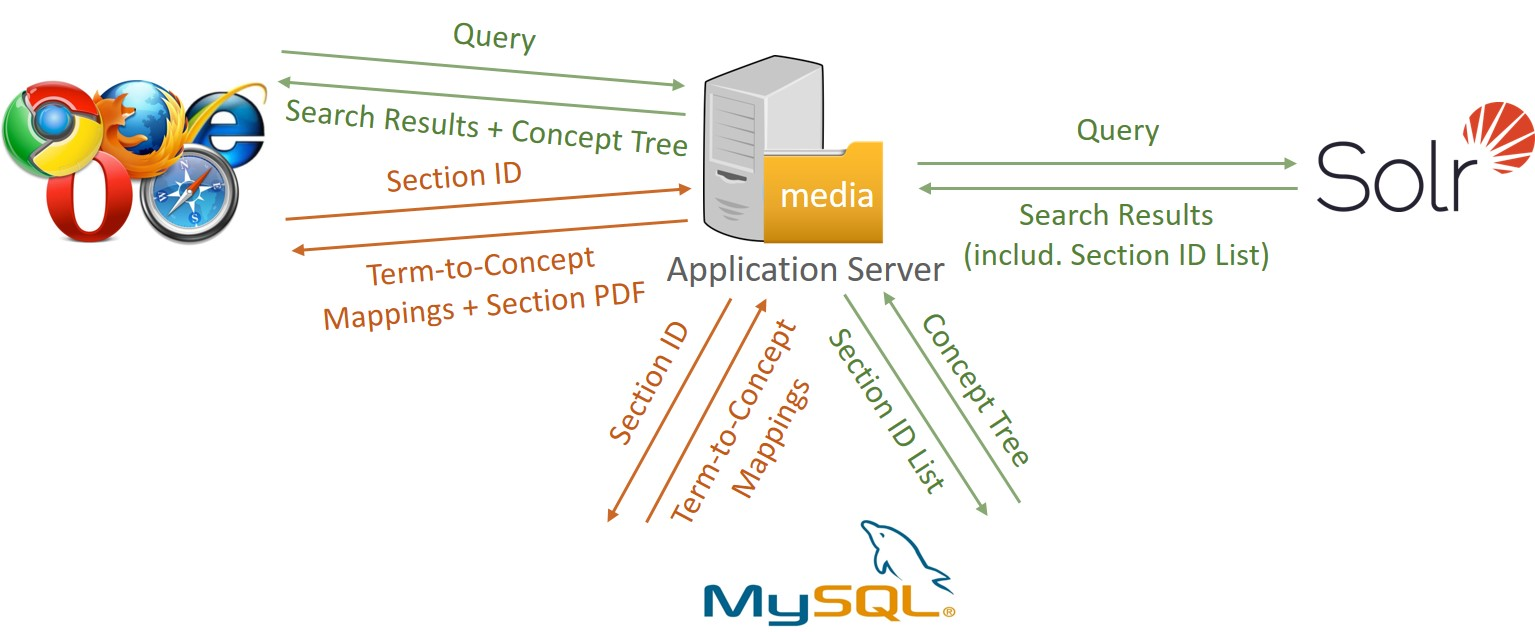
\includegraphics[width=.9\textwidth]{proposed_methodology_and_system_specifications/component_searching.jpg}
  \caption{Component for Searching and Viewing}
  \label{fig:comp_search}
\end{figure}

\begin{itemize}
\item \textbf{Searching:} Users send a query to the Application Server. The Application Server passes the query to the search engine Solr and then receives the search results from Solr. The search results are a list of documents (i.e. sections) with meta-data including section ID, book, and page number. Next, the Application Server requests for all concepts identified in search results from MySQL. Finally, the Application Server responds to users by sending back the search results and the concept tree. The concept tree consists of concept nodes which map to one or more terms in the documents from the search results.

\item \textbf{Viewing:} Users request to view one document from the search results. The Application Server receives the section ID. It then retrieves the PDF from the \texttt{Media} folder and the term-to-concept mappings for this section from MySQL. Finally, it responds to users by sending back the term-to-concept mappings and the PDF for that document.
\end{itemize}
